\documentclass[tikz,border=2pt]{standalone}
\usepackage{amsmath}
\usetikzlibrary{arrows.meta}
\begin{document}
% A loss X = 1000 with coinsurance a = 0.8 and deductible d = 100, split between insured and insurer
% in the two orders: a(X-d)_+ = 720 (insured 280) versus (aX-d)_+ = 700 (insured 300).
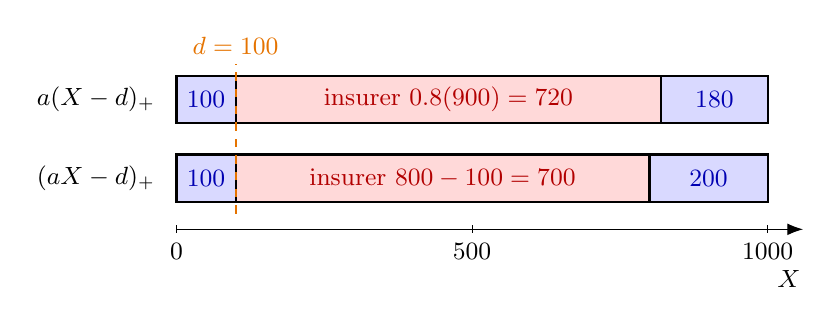
\begin{tikzpicture}[font=\small, >={Latex[length=2mm]}, x=0.0075cm, y=1cm]
  \def\bh{0.6}
  % top bar: deductible first, then share
  \fill[blue!15] (0,1) rectangle (100,1+\bh);
  \fill[red!15] (100,1) rectangle (820,1+\bh);
  \fill[blue!15] (820,1) rectangle (1000,1+\bh);
  \draw[thick] (0,1) rectangle (1000,1+\bh);
  \draw[thick] (100,1) -- (100,1+\bh);
  \draw[thick] (820,1) -- (820,1+\bh);
  \node[blue!70!black] at (50,1+0.5*\bh) {$100$};
  \node[red!70!black] at (460,1+0.5*\bh) {insurer $0.8(900)=720$};
  \node[blue!70!black] at (910,1+0.5*\bh) {$180$};
  \node[anchor=east] at (-20,1+0.5*\bh) {$a(X-d)_+$};
  % bottom bar: share first, then deductible
  \fill[blue!15] (0,0) rectangle (100,\bh);
  \fill[red!15] (100,0) rectangle (800,\bh);
  \fill[blue!15] (800,0) rectangle (1000,\bh);
  \draw[thick] (0,0) rectangle (1000,\bh);
  \draw[thick] (100,0) -- (100,\bh);
  \draw[thick] (800,0) -- (800,\bh);
  \node[blue!70!black] at (50,0.5*\bh) {$100$};
  \node[red!70!black] at (450,0.5*\bh) {insurer $800-100=700$};
  \node[blue!70!black] at (900,0.5*\bh) {$200$};
  \node[anchor=east] at (-20,0.5*\bh) {$(aX-d)_+$};
  % deductible marker and loss scale
  \draw[orange!90!black, thick, dashed] (100,-0.15) -- (100,1.75);
  \node[orange!90!black, anchor=south] at (100,1.75) {$d=100$};
  \draw[->] (0,-0.35) -- (1060,-0.35);
  \foreach \t in {0,500,1000} {\draw (\t,-0.3) -- (\t,-0.4) node[below] {$\t$};}
  \node[anchor=north west] at (1000,-0.75) {$X$};
\end{tikzpicture}
\end{document}
